\documentclass[12pt,a4paper]{article}
\usepackage[UTF8]{ctex}
\usepackage{amsmath}
\usepackage{amssymb}
\usepackage{amsthm}
\usepackage{graphicx}
\usepackage{hyperref}
\usepackage{geometry}
\usepackage{algorithm}
\usepackage{algorithmic}
\usepackage{listings}
\usepackage{xcolor}
\usepackage{fancyhdr}
\geometry{left=2cm,right=2cm,top=2.5cm,bottom=2.5cm,headheight=15pt}
\setlength{\baselineskip}{1.1\baselineskip}
\setlength{\parskip}{0.5em}

% 导入通用样式
% 通用样式文件 - 统一所有文档的样式

% 目录样式设置 - 干净简洁,无边框,优化编号
% 使用基本 LaTeX 命令美化目录
\makeatletter
\renewcommand\@dotsep{2}
% 优化编号格式:减少缩进,使编号更紧凑
\renewcommand\l@section{\@dottedtocline{1}{0em}{1.2em}}
\renewcommand\l@subsection{\@dottedtocline{2}{1.2em}{1.8em}}
\renewcommand\l@subsubsection{\@dottedtocline{3}{3em}{2.2em}}
% 设置目录深度为3,显示到subsubsection级别
\setcounter{tocdepth}{3}
\makeatother

% 超链接设置 - 目录链接无颜色框
\hypersetup{
    colorlinks=true,
    linkcolor=black,          % 目录链接为黑色
    filecolor=black,
    urlcolor=blue,
    citecolor=black,
    pdfstartview=FitH,
    pdfborder={0 0 0},        % 无边框
    linkbordercolor={0 0 0},  % 链接边框颜色为黑色(不可见)
    pdfborderstyle={/S/U},    % 无边框样式
}

% 页眉页脚设置(在文档中重新定义)
\usepackage{fancyhdr}
% 注意:每个文档需要在导入 common_style.tex 后设置自己的页眉页脚

% 章节格式 - 简洁美观(使用基本命令)
\makeatletter
\renewcommand\section{\@startsection {section}{1}{\z@}%
                                   {-3.5ex \@plus -1ex \@minus -.2ex}%
                                   {2.3ex \@plus.2ex}%
                                   {\normalfont\Large\bfseries}}
\renewcommand\subsection{\@startsection{subsection}{2}{\z@}%
                                     {-3.25ex\@plus -1ex \@minus -.2ex}%
                                     {1.5ex \@plus .2ex}%
                                     {\normalfont\large\bfseries}}
\renewcommand\subsubsection{\@startsection{subsubsection}{3}{\z@}%
                                     {-3.25ex\@plus -1ex \@minus -.2ex}%
                                     {1.5ex \@plus .2ex}%
                                     {\normalfont\normalsize\bfseries}}
\makeatother

% 代码样式设置 - 简洁干净,无背景色
\definecolor{codegray}{rgb}{0.5,0.5,0.5}
\definecolor{keywordblue}{rgb}{0,0,0.8}
\definecolor{stringred}{rgb}{0.3,0.3,0.3}
\definecolor{commentgreen}{rgb}{0,0.5,0}

\lstdefinestyle{pythonstyle}{
    language=Python,
    % 无背景色 - 使用白色背景,与文档背景一致
    commentstyle=\color{commentgreen},      % 注释不用斜体
    keywordstyle=\color{keywordblue}\bfseries,
    stringstyle=\color{stringred},
    basicstyle=\ttfamily\small,
    breakatwhitespace=false,
    breaklines=true,
    captionpos=b,
    keepspaces=true,
    numbers=none,                           % 不显示行号
    showspaces=false,
    showstringspaces=false,
    showtabs=false,
    tabsize=4,
    frame=single,                          % 保留边框,但更简洁
    rulecolor=\color{black},
    framerule=0.5pt,                       % 细边框
    framexleftmargin=8pt,                  % 左边距(代码与左边框的距离)
    framexrightmargin=8pt,                 % 右边距(代码与右边框的距离)
    framextopmargin=6pt,                   % 上边距(代码与上边框的距离)
    framexbottommargin=6pt,                % 下边距(代码与下边框的距离)
    morekeywords={import,from,as,class,def,return,yield,lambda,if,elif,else,for,while,break,continue,pass,try,except,finally,raise,assert,with,del,global,nonlocal,and,or,not,in,is},
    identifierstyle=\color{black},
}

\lstset{style=pythonstyle}

% 封面宏定义
\newcommand{\makecover}[5]{%
    \newpage
    \thispagestyle{empty}
    \vspace*{1.5cm}
    \begin{center}
        \vspace{2cm}
        {\fontsize{48}{58}\selectfont\bfseries #1}\\[0.8cm]
        \vspace{1.5cm}
        {\Large #2}\\[0.4cm]
        \vspace{1.5cm}
        {\large #3}\\[1.5cm]
        
        % 神经网络图 - 紧凑版本,无标签
        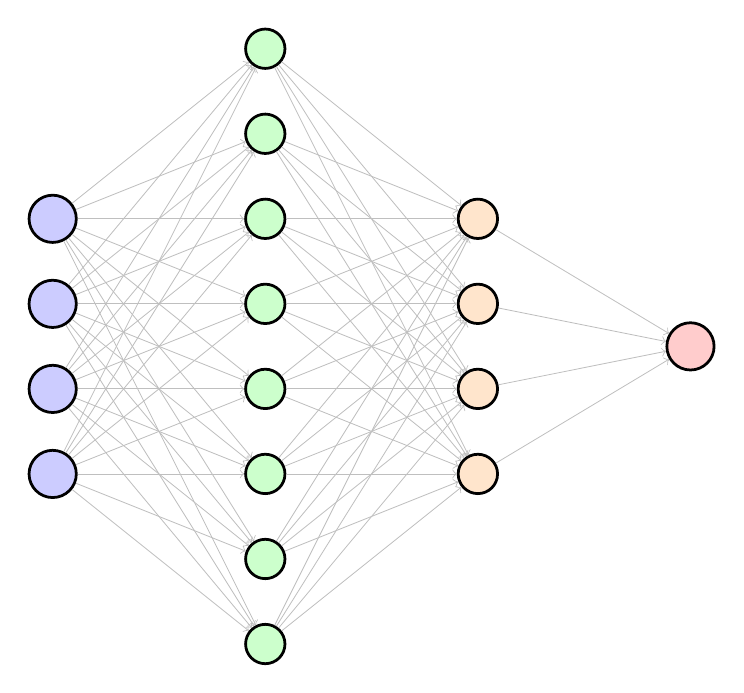
\begin{tikzpicture}[scale=0.9]
        % 定义神经元间距
        \def\spacing{1.2}
        
        % 输入层 - 4个神经元,关于横轴对称
        \node[circle, draw, minimum size=0.6cm, fill=blue!20, line width=1pt] (x1) at (0, -1.8) {};
        \node[circle, draw, minimum size=0.6cm, fill=blue!20, line width=1pt] (x2) at (0, -0.6) {};
        \node[circle, draw, minimum size=0.6cm, fill=blue!20, line width=1pt] (x3) at (0, 0.6) {};
        \node[circle, draw, minimum size=0.6cm, fill=blue!20, line width=1pt] (x4) at (0, 1.8) {};
        
        % 隐藏层1 - 8个神经元,关于横轴对称
        \node[circle, draw, minimum size=0.5cm, fill=green!20, line width=1pt] (h11) at (3, -4.2) {};
        \node[circle, draw, minimum size=0.5cm, fill=green!20, line width=1pt] (h12) at (3, -3.0) {};
        \node[circle, draw, minimum size=0.5cm, fill=green!20, line width=1pt] (h13) at (3, -1.8) {};
        \node[circle, draw, minimum size=0.5cm, fill=green!20, line width=1pt] (h14) at (3, -0.6) {};
        \node[circle, draw, minimum size=0.5cm, fill=green!20, line width=1pt] (h15) at (3, 0.6) {};
        \node[circle, draw, minimum size=0.5cm, fill=green!20, line width=1pt] (h16) at (3, 1.8) {};
        \node[circle, draw, minimum size=0.5cm, fill=green!20, line width=1pt] (h17) at (3, 3.0) {};
        \node[circle, draw, minimum size=0.5cm, fill=green!20, line width=1pt] (h18) at (3, 4.2) {};
        
        % 隐藏层2 - 4个神经元,关于横轴对称
        \node[circle, draw, minimum size=0.5cm, fill=orange!20, line width=1pt] (h21) at (6, -1.8) {};
        \node[circle, draw, minimum size=0.5cm, fill=orange!20, line width=1pt] (h22) at (6, -0.6) {};
        \node[circle, draw, minimum size=0.5cm, fill=orange!20, line width=1pt] (h23) at (6, 0.6) {};
        \node[circle, draw, minimum size=0.5cm, fill=orange!20, line width=1pt] (h24) at (6, 1.8) {};
        
        % 输出层 - 1个神经元,在横轴上
        \node[circle, draw, minimum size=0.6cm, fill=red!20, line width=1pt] (y) at (9, 0) {};
        
        % 输入层到隐藏层1的连接
        \foreach \i in {1,...,4}
            \foreach \j in {1,...,8}
                \draw[->, gray!50, line width=0.3pt] (x\i) -- (h1\j);
        
        % 隐藏层1到隐藏层2的连接
        \foreach \i in {1,...,8}
            \foreach \j in {1,...,4}
                \draw[->, gray!50, line width=0.3pt] (h1\i) -- (h2\j);
        
        % 隐藏层2到输出层的连接
        \foreach \i in {1,...,4}
            \draw[->, gray!50, line width=0.3pt] (h2\i) -- (y);
        \end{tikzpicture}
        
        \vfill
        \vspace{2cm}
        {\normalsize #5}
        \vspace{1.5cm}
    \end{center}
    \newpage
}



% 页眉页脚设置
\pagestyle{fancy}
\fancyhf{}
\fancyhead[L]{\leftmark}
\fancyhead[R]{\thepage}
\fancyfoot[C]{\small Python、NumPy 和 Pandas 核心知识与应用}
\renewcommand{\headrulewidth}{0.3pt}
\renewcommand{\footrulewidth}{0.3pt}

\title{Python、NumPy 和 Pandas 核心知识与应用}
\author{}
\date{\today}

\newtheorem{definition}{定义}[section]
\newtheorem{example}{例}[section]
\newtheorem{remark}{注}[section]

\begin{document}

% 封面
\makecover{Python、NumPy 和 Pandas\\核心知识与应用}{Python 基础 · NumPy 数值计算 · Pandas 数据处理}{数据科学与机器学习的必备工具集}{AI/ML 系列教程}

\maketitle

\tableofcontents
\newpage

\section{引言}

Python 是数据科学和机器学习领域最流行的编程语言,其简洁的语法、丰富的生态系统和强大的数据处理能力使其成为 AI/ML 研究的首选工具。NumPy 提供了高效的数值计算基础,Pandas 则提供了强大的数据分析和处理能力。三者结合构成了现代数据科学工作流的核心工具链。

\textbf{Python、NumPy、Pandas 在数据科学工作流中的重要性}:
\begin{itemize}
    \item \textbf{数据获取与清洗}:Pandas 提供了强大的数据读取、清洗和预处理能力
    \item \textbf{数值计算}:NumPy 提供了高效的数组操作和数学运算
    \item \textbf{特征工程}:Python 的灵活性和 Pandas 的数据操作能力使特征工程变得简单
    \item \textbf{模型训练}:NumPy 数组是大多数机器学习库(如 scikit-learn、PyTorch)的底层数据结构
    \item \textbf{结果分析}:Pandas 提供了丰富的数据分析和可视化工具
\end{itemize}

本文档分为两部分:第一部分介绍 Python 基础语法和 NumPy 核心功能;第二部分介绍 Pandas 数据处理和分析。

\part{第一部分:Python 基础与 NumPy}

\section{Python 基础语法}

\subsection{变量与数据类型}

\textbf{概念解释}:Python 是动态类型语言,变量不需要显式声明类型,类型在运行时确定。

\textbf{基本数据类型}:
\begin{itemize}
    \item \textbf{整数(int)}:任意大小的整数
    \item \textbf{浮点数(float)}:双精度浮点数
    \item \textbf{字符串(str)}:不可变字符序列
    \item \textbf{布尔值(bool)}:True 或 False
    \item \textbf{列表(list)}:可变有序序列
    \item \textbf{元组(tuple)}:不可变有序序列
    \item \textbf{字典(dict)}:键值对映射
    \item \textbf{集合(set)}:无序不重复元素集
\end{itemize}

\begin{lstlisting}[caption=Python 基本数据类型示例]
# 整数
x = 42
print(type(x))  # <class 'int'>

# 浮点数
y = 3.14
print(type(y))  # <class 'float'>

# 字符串
name = "Python"
print(type(name))  # <class 'str'>

# 列表
numbers = [1, 2, 3, 4, 5]
print(type(numbers))  # <class 'list'>

# 字典
person = {"name": "Alice", "age": 30}
print(type(person))  # <class 'dict'>

# 集合
unique_numbers = {1, 2, 3, 4, 5}
print(type(unique_numbers))  # <class 'set'>
\end{lstlisting}

\textbf{在 AI/ML 中的应用}:
\begin{itemize}
    \item 列表用于存储特征向量、样本索引等
    \item 字典用于存储模型参数、配置信息
    \item 字符串用于处理文本数据、文件路径
\end{itemize}

\subsection{控制流}

\textbf{条件语句}:
\begin{lstlisting}[caption=条件语句示例]
# if-elif-else
score = 85

if score >= 90:
    grade = "A"
elif score >= 80:
    grade = "B"
elif score >= 70:
    grade = "C"
else:
    grade = "D"

print(f"分数 {score} 对应的等级是 {grade}")

# 在数据处理中的应用:数据分类
def categorize_age(age):
    if age < 18:
        return "未成年"
    elif age < 65:
        return "成年"
    else:
        return "老年"
\end{lstlisting}

\textbf{循环语句}:
\begin{lstlisting}[caption=循环语句示例]
# for 循环
numbers = [1, 2, 3, 4, 5]
squared = []
for num in numbers:
    squared.append(num ** 2)
print(squared)  # [1, 4, 9, 16, 25]

# while 循环
count = 0
while count < 5:
    print(count)
    count += 1

# 在数据处理中的应用:遍历数据
data = [{"name": "Alice", "age": 25}, {"name": "Bob", "age": 30}]
for person in data:
    print(f"{person['name']} is {person['age']} years old")
\end{lstlisting}

\subsection{函数定义}

\textbf{概念解释}:函数是组织代码的基本单元,可以接受参数并返回结果。

\begin{lstlisting}[caption=函数定义示例]
# 基本函数定义
def add(a, b):
    """计算两个数的和"""
    return a + b

result = add(3, 5)
print(result)  # 8

# 默认参数
def greet(name, greeting="Hello"):
    """打招呼函数,带有默认参数"""
    return f"{greeting}, {name}!"

print(greet("Alice"))  # Hello, Alice!
print(greet("Bob", "Hi"))  # Hi, Bob!

# 可变参数
def sum_all(*args):
    """计算所有参数的和"""
    total = 0
    for num in args:
        total += num
    return total

print(sum_all(1, 2, 3, 4, 5))  # 15

# 关键字参数
def create_person(name, age, **kwargs):
    """创建人员信息字典"""
    person = {"name": name, "age": age}
    person.update(kwargs)
    return person

person = create_person("Alice", 25, city="Beijing", job="Engineer")
print(person)  # {'name': 'Alice', 'age': 25, 'city': 'Beijing', 'job': 'Engineer'}
\end{lstlisting}

\textbf{在 AI/ML 中的应用}:
\begin{itemize}
    \item 定义数据预处理函数
    \item 实现评估指标函数
    \item 封装模型训练流程
\end{itemize}

\subsection{面向对象编程}

\textbf{概念解释}:面向对象编程(OOP)通过类和对象组织代码,实现封装、继承和多态。

\textbf{类与对象}:
\begin{lstlisting}[caption=类定义示例]
class Dataset:
    """数据集类,用于管理机器学习数据"""
    
    def __init__(self, data, labels=None):
        """
        初始化数据集
        
        参数:
            data: 特征数据
            labels: 标签数据(可选)
        """
        self.data = data
        self.labels = labels
        self.size = len(data)
    
    def __len__(self):
        """返回数据集大小"""
        return self.size
    
    def __getitem__(self, index):
        """支持索引访问"""
        if self.labels is not None:
            return self.data[index], self.labels[index]
        return self.data[index]
    
    def get_batch(self, batch_size):
        """获取一个批次的数据"""
        indices = list(range(0, self.size, batch_size))
        for i in indices:
            end = min(i + batch_size, self.size)
            if self.labels is not None:
                yield self.data[i:end], self.labels[i:end]
            else:
                yield self.data[i:end]

# 使用示例
data = [[1, 2], [3, 4], [5, 6]]
labels = [0, 1, 0]
dataset = Dataset(data, labels)

print(f"数据集大小: {len(dataset)}")  # 数据集大小: 3
print(f"第一个样本: {dataset[0]}")  # 第一个样本: ([1, 2], 0)

# 获取批次
for batch_data, batch_labels in dataset.get_batch(2):
    print(f"批次数据: {batch_data}, 批次标签: {batch_labels}")
\end{lstlisting}

\textbf{继承}:
\begin{lstlisting}[caption=继承示例]
class BaseModel:
    """基础模型类"""
    
    def __init__(self):
        self.trained = False
    
    def train(self):
        """训练模型"""
        self.trained = True
        print("模型训练完成")
    
    def predict(self, x):
        """预测(需要在子类中实现)"""
        raise NotImplementedError("子类必须实现 predict 方法")

class LinearModel(BaseModel):
    """线性模型,继承自 BaseModel"""
    
    def __init__(self):
        super().__init__()
        self.weights = None
    
    def train(self, X, y):
        """训练线性模型"""
        # 简化的训练过程
        self.weights = [0.5, 0.3]  # 示例权重
        super().train()
    
    def predict(self, x):
        """预测"""
        if not self.trained:
            raise ValueError("模型尚未训练")
        # 简化的预测:w0 * x[0] + w1 * x[1]
        return self.weights[0] * x[0] + self.weights[1] * x[1]

# 使用示例
model = LinearModel()
model.train([[1, 2], [3, 4]], [1, 2])
prediction = model.predict([2, 3])
print(f"预测结果: {prediction}")
\end{lstlisting}

\subsection{常用内置模块}

\textbf{os 模块}:操作系统接口
\begin{lstlisting}[caption=os 模块示例]
import os

# 获取当前工作目录
current_dir = os.getcwd()
print(f"当前目录: {current_dir}")

# 列出目录内容
files = os.listdir('.')
print(f"目录内容: {files}")

# 检查文件是否存在
file_path = "data.csv"
if os.path.exists(file_path):
    print(f"{file_path} 存在")
else:
    print(f"{file_path} 不存在")

# 路径操作
base_path = "/home/user"
data_path = os.path.join(base_path, "data", "dataset.csv")
print(f"完整路径: {data_path}")
\end{lstlisting}

\textbf{json 模块}:JSON 数据处理
\begin{lstlisting}[caption=json 模块示例]
import json

# 将 Python 对象转换为 JSON 字符串
data = {
    "name": "Alice",
    "age": 25,
    "scores": [85, 90, 88]
}
json_string = json.dumps(data, ensure_ascii=False, indent=2)
print(json_string)

# 将 JSON 字符串转换为 Python 对象
parsed_data = json.loads(json_string)
print(parsed_data["name"])

# 读写 JSON 文件
# 写入
with open("data.json", "w", encoding="utf-8") as f:
    json.dump(data, f, ensure_ascii=False, indent=2)

# 读取
with open("data.json", "r", encoding="utf-8") as f:
    loaded_data = json.load(f)
    print(loaded_data)
\end{lstlisting}

\textbf{datetime 模块}:日期时间处理
\begin{lstlisting}[caption=datetime 模块示例]
from datetime import datetime, timedelta

# 获取当前时间
now = datetime.now()
print(f"当前时间: {now}")

# 格式化时间
formatted = now.strftime("%Y-%m-%d %H:%M:%S")
print(f"格式化时间: {formatted}")

# 解析时间字符串
time_str = "2024-01-15 10:30:00"
parsed_time = datetime.strptime(time_str, "%Y-%m-%d %H:%M:%S")
print(f"解析的时间: {parsed_time}")

# 时间计算
future_time = now + timedelta(days=7)
print(f"7天后: {future_time}")

# 在时间序列数据处理中的应用
dates = [datetime(2024, 1, i) for i in range(1, 6)]
print("日期列表:", dates)
\end{lstlisting}

\textbf{collections 模块}:特殊容器类型
\begin{lstlisting}[caption=collections 模块示例]
from collections import Counter, defaultdict, deque

# Counter: 计数器
words = ["apple", "banana", "apple", "orange", "banana", "apple"]
word_count = Counter(words)
print(f"词频统计: {word_count}")
print(f"最常见的2个: {word_count.most_common(2)}")

# defaultdict: 带默认值的字典
dd = defaultdict(list)
dd["fruits"].append("apple")
dd["fruits"].append("banana")
print(f"默认字典: {dict(dd)}")

# deque: 双端队列
queue = deque([1, 2, 3])
queue.append(4)  # 右端添加
queue.appendleft(0)  # 左端添加
print(f"双端队列: {queue}")
\end{lstlisting}

\subsection{文件操作}

\textbf{CSV 文件处理}:
\begin{lstlisting}[caption=CSV 文件处理示例]
import csv

# 写入 CSV 文件
data = [
    ["姓名", "年龄", "城市"],
    ["Alice", 25, "北京"],
    ["Bob", 30, "上海"],
    ["Charlie", 35, "广州"]
]

with open("people.csv", "w", newline="", encoding="utf-8") as f:
    writer = csv.writer(f)
    writer.writerows(data)

# 读取 CSV 文件
with open("people.csv", "r", encoding="utf-8") as f:
    reader = csv.reader(f)
    header = next(reader)  # 读取表头
    print(f"表头: {header}")
    for row in reader:
        print(f"数据: {row}")

# 使用字典方式读写(更常用)
with open("people.csv", "r", encoding="utf-8") as f:
    reader = csv.DictReader(f)
    for row in reader:
        print(f"姓名: {row['姓名']}, 年龄: {row['年龄']}")
\end{lstlisting}

\textbf{异常处理}:
\begin{lstlisting}[caption=异常处理示例]
# 基本异常处理
try:
    result = 10 / 0
except ZeroDivisionError:
    print("除数不能为零!")

# 多个异常类型
try:
    value = int("abc")
    result = 10 / value
except ValueError:
    print("无法转换为整数")
except ZeroDivisionError:
    print("除数不能为零")
except Exception as e:
    print(f"发生错误: {e}")

# finally 子句
def read_file_safely(filename):
    """安全读取文件"""
    try:
        with open(filename, "r", encoding="utf-8") as f:
            content = f.read()
        return content
    except FileNotFoundError:
        print(f"文件 {filename} 不存在")
        return None
    except Exception as e:
        print(f"读取文件时出错: {e}")
        return None
    finally:
        print("文件操作完成")

# 自定义异常
class DataValidationError(Exception):
    """数据验证错误"""
    pass

def validate_age(age):
    """验证年龄"""
    if age < 0 or age > 150:
        raise DataValidationError(f"年龄 {age} 不在有效范围内")
    return True

try:
    validate_age(200)
except DataValidationError as e:
    print(f"验证失败: {e}")
\end{lstlisting}

\subsection{高级特性}

\textbf{列表推导式}:
\begin{lstlisting}[caption=列表推导式示例]
# 基本列表推导式
squares = [x**2 for x in range(10)]
print(f"平方数: {squares}")

# 带条件的列表推导式
even_squares = [x**2 for x in range(10) if x % 2 == 0]
print(f"偶数的平方: {even_squares}")

# 嵌套列表推导式
matrix = [[i*j for j in range(3)] for i in range(3)]
print(f"矩阵: {matrix}")

# 在数据处理中的应用:特征提取
data = [{"age": 25, "score": 85}, {"age": 30, "score": 90}]
ages = [person["age"] for person in data]
scores = [person["score"] for person in data if person["score"] > 80]
print(f"年龄列表: {ages}")
print(f"高分列表: {scores}")
\end{lstlisting}

\textbf{生成器}:
\begin{lstlisting}[caption=生成器示例]
# 生成器函数
def fibonacci(n):
    """生成斐波那契数列"""
    a, b = 0, 1
    count = 0
    while count < n:
        yield a
        a, b = b, a + b
        count += 1

# 使用生成器
for num in fibonacci(10):
    print(num, end=" ")
print()

# 生成器表达式
squares_gen = (x**2 for x in range(10))
print(f"生成器对象: {squares_gen}")
print(f"转换为列表: {list(squares_gen)}")

# 在数据处理中的应用:大数据流处理
def read_large_file(filename):
    """逐行读取大文件"""
    with open(filename, "r", encoding="utf-8") as f:
        for line in f:
            yield line.strip()

# 使用生成器处理大文件,节省内存
# for line in read_large_file("large_data.txt"):
#     process(line)
\end{lstlisting}

\textbf{装饰器}:
\begin{lstlisting}[caption=装饰器示例]
import time
from functools import wraps

# 基本装饰器
def timer(func):
    """计时装饰器"""
    @wraps(func)
    def wrapper(*args, **kwargs):
        start = time.time()
        result = func(*args, **kwargs)
        end = time.time()
        print(f"{func.__name__} 执行时间: {end - start:.4f} 秒")
        return result
    return wrapper

@timer
def slow_function():
    """慢速函数"""
    time.sleep(1)
    return "完成"

result = slow_function()

# 带参数的装饰器
def repeat(times):
    """重复执行装饰器"""
    def decorator(func):
        @wraps(func)
        def wrapper(*args, **kwargs):
            results = []
            for _ in range(times):
                results.append(func(*args, **kwargs))
            return results
        return wrapper
    return decorator

@repeat(3)
def greet(name):
    return f"Hello, {name}!"

print(greet("Alice"))
\end{lstlisting}

\section{NumPy 基础}

NumPy(Numerical Python)是 Python 科学计算的基础库,提供了高效的多维数组对象和数学运算函数。

\subsection{NumPy 基础概念}

\textbf{概念解释}:
\begin{itemize}
    \item \textbf{数组(ndarray)}:NumPy 的核心数据结构,是同质多维数组
    \item \textbf{维度(dimension)}:数组的轴数,1维数组有1个轴,2维数组有2个轴
    \item \textbf{形状(shape)}:描述数组每个维度大小的元组
    \item \textbf{数据类型(dtype)}:数组中元素的数据类型
\end{itemize}

\textbf{学术解释}:NumPy 数组是连续内存块中的同质数据集合,支持向量化操作,比 Python 列表快数十到数百倍。

\textbf{通俗解释}:NumPy 数组就像一个整齐排列的表格,所有数据都是同一种类型,可以快速进行数学运算。

\subsection{数组创建与初始化}

\begin{lstlisting}[caption=数组创建示例]
import numpy as np

# 从列表创建数组
arr1 = np.array([1, 2, 3, 4, 5])
print(f"一维数组: {arr1}")
print(f"形状: {arr1.shape}")  # (5,)
print(f"维度: {arr1.ndim}")  # 1
print(f"数据类型: {arr1.dtype}")  # int64

# 二维数组
arr2 = np.array([[1, 2, 3], [4, 5, 6]])
print(f"二维数组:\n{arr2}")
print(f"形状: {arr2.shape}")  # (2, 3)

# 创建全零数组
zeros = np.zeros((3, 4))
print(f"全零数组:\n{zeros}")

# 创建全一数组
ones = np.ones((2, 3))
print(f"全一数组:\n{ones}")

# 创建单位矩阵
identity = np.eye(3)
print(f"单位矩阵:\n{identity}")

# 使用 arange 创建数组
arr_range = np.arange(0, 10, 2)
print(f"arange(0, 10, 2): {arr_range}")  # [0 2 4 6 8]

# 使用 linspace 创建等间距数组
arr_linspace = np.linspace(0, 1, 5)
print(f"linspace(0, 1, 5): {arr_linspace}")  # [0.   0.25 0.5  0.75 1.  ]

# 随机数组
random_arr = np.random.rand(3, 3)  # [0, 1) 均匀分布
print(f"随机数组:\n{random_arr}")

normal_arr = np.random.randn(3, 3)  # 标准正态分布
print(f"正态分布随机数组:\n{normal_arr}")

# 指定数据类型的数组
int_arr = np.array([1, 2, 3], dtype=np.float32)
print(f"浮点数组: {int_arr}, 类型: {int_arr.dtype}")
\end{lstlisting}

\textbf{API 说明}:
\begin{itemize}
    \item \texttt{np.array(object, dtype=None)}:从列表或其他数组创建数组
    \item \texttt{np.zeros(shape, dtype=float)}:创建全零数组
    \item \texttt{np.ones(shape, dtype=float)}:创建全一数组
    \item \texttt{np.arange(start, stop, step)}:创建等间距数组
    \item \texttt{np.linspace(start, stop, num)}:创建指定数量的等间距数组
    \item \texttt{np.random.rand(*dims)}:创建 [0,1) 均匀分布随机数组
    \item \texttt{np.random.randn(*dims)}:创建标准正态分布随机数组
\end{itemize}

\subsection{数组操作}

\textbf{索引与切片}:

\textbf{概念解释}:索引用于访问数组的特定元素,切片用于获取数组的子数组。

\textbf{数学表达式演示}:

对于矩阵 $\mathbf{A} \in \mathbb{R}^{m \times n}$:
\begin{equation}
\mathbf{A} = \begin{bmatrix}
A_{00} & A_{01} & A_{02} & A_{03} \\
A_{10} & A_{11} & A_{12} & A_{13} \\
A_{20} & A_{21} & A_{22} & A_{23}
\end{bmatrix}
\end{equation}

\textbf{基本索引}:访问第 $i$ 行第 $j$ 列的元素:
\begin{equation}
A_{ij} = \mathbf{A}[i, j]
\end{equation}

\textbf{切片操作}:
\begin{itemize}
    \item 第 $i$ 行:$\mathbf{A}[i, :] = [A_{i0}, A_{i1}, A_{i2}, A_{i3}]$
    \item 第 $j$ 列:$\mathbf{A}[:, j] = [A_{0j}, A_{1j}, A_{2j}]^T$
    \item 前 $k$ 行:$\mathbf{A}[:k, :] = \begin{bmatrix} A_{00} & \cdots & A_{0(n-1)} \\ \vdots & \ddots & \vdots \\ A_{(k-1)0} & \cdots & A_{(k-1)(n-1)} \end{bmatrix}$
\end{itemize}

\textbf{布尔索引}:对于条件 $C(\mathbf{A})$,布尔索引定义为:
\begin{equation}
\mathbf{A}[C(\mathbf{A})] = \{A_{ij} : C(A_{ij}) = \text{True}\}
\end{equation}

例如,$C(x) = x > 5$,则:
\begin{equation}
\mathbf{A}[\mathbf{A} > 5] = \{A_{ij} : A_{ij} > 5\}
\end{equation}

\begin{lstlisting}[caption=数组索引与切片示例]
import numpy as np

arr = np.array([[1, 2, 3, 4],
                [5, 6, 7, 8],
                [9, 10, 11, 12]])

print("原始数组:")
print(arr)
# [[ 1  2  3  4]
#  [ 5  6  7  8]
#  [ 9 10 11 12]]

# 基本索引
print(f"\narr[0, 0] = {arr[0, 0]}")  # 1
print(f"arr[1, 2] = {arr[1, 2]}")  # 7

# 切片
print(f"\n第一行 arr[0, :] = {arr[0, :]}")  # [1 2 3 4]
print(f"第一列 arr[:, 0] = {arr[:, 0]}")  # [1 5 9]
print(f"\n前两行 arr[:2, :]:\n{arr[:2, :]}")
# [[1 2 3 4]
#  [5 6 7 8]]
print(f"\n前两列 arr[:, :2]:\n{arr[:, :2]}")
# [[ 1  2]
#  [ 5  6]
#  [ 9 10]]

# 布尔索引
mask = arr > 5
print(f"\n布尔掩码 (arr > 5):\n{mask}")
# [[False False False False]
#  [False  True  True  True]
#  [ True  True  True  True]]
print(f"\n大于5的值 arr[mask] = {arr[mask]}")  # [6 7 8 9 10 11 12]

# 花式索引(Fancy Indexing)
indices = [0, 2]
print(f"\n选择第0和第2行 arr[[0, 2], :]:\n{arr[indices, :]}")
# [[ 1  2  3  4]
#  [ 9 10 11 12]]
\end{lstlisting}

\textbf{数组重塑与转置}:

\textbf{概念解释}:重塑(reshape)改变数组的形状而不改变数据,转置(transpose)交换数组的维度。

\textbf{数学表达式演示}:

对于一维数组 $\mathbf{a} = [a_0, a_1, \ldots, a_{11}]$,重塑为 $3 \times 4$ 矩阵:
\begin{equation}
\mathbf{a} = [a_0, a_1, a_2, a_3, a_4, a_5, a_6, a_7, a_8, a_9, a_{10}, a_{11}]^T
\end{equation}

重塑为 $3 \times 4$ 矩阵:
\begin{equation}
\text{reshape}(\mathbf{a}, (3, 4)) = \begin{bmatrix}
a_0 & a_1 & a_2 & a_3 \\
a_4 & a_5 & a_6 & a_7 \\
a_8 & a_9 & a_{10} & a_{11}
\end{bmatrix} = \mathbf{A}
\end{equation}

转置操作:
\begin{equation}
\mathbf{A}^T = \begin{bmatrix}
a_0 & a_4 & a_8 \\
a_1 & a_5 & a_9 \\
a_2 & a_6 & a_{10} \\
a_3 & a_7 & a_{11}
\end{bmatrix}
\end{equation}

对于矩阵 $\mathbf{A} \in \mathbb{R}^{m \times n}$,转置定义为:
\begin{equation}
(\mathbf{A}^T)_{ij} = A_{ji}
\end{equation}

\begin{lstlisting}[caption=数组重塑示例]
import numpy as np

arr = np.arange(12)
print(f"原始数组: {arr}")  # [0 1 2 3 4 5 6 7 8 9 10 11]

# 重塑为 3x4 数组
reshaped = arr.reshape(3, 4)
print(f"重塑为 3x4:\n{reshaped}")
# [[ 0  1  2  3]
#  [ 4  5  6  7]
#  [ 8  9 10 11]]

# 转置
transposed = reshaped.T
print(f"转置:\n{transposed}")
# [[ 0  4  8]
#  [ 1  5  9]
#  [ 2  6 10]
#  [ 3  7 11]]

# 展平
flattened = reshaped.flatten()
print(f"展平: {flattened}")  # [0 1 2 3 4 5 6 7 8 9 10 11]

# 改变形状(不复制数据)
arr_2d = arr.reshape(3, 4)
arr_2d[0, 0] = 999
print(f"修改后原数组: {arr}")  # 原数组也被修改
\end{lstlisting}

\textbf{数组拼接}:

\textbf{概念解释}:拼接(concatenation)将多个数组沿指定轴组合成一个数组。

\textbf{数学表达式演示}:

对于矩阵 $\mathbf{A} = \begin{bmatrix} 1 & 2 \\ 3 & 4 \end{bmatrix}$ 和 $\mathbf{B} = \begin{bmatrix} 5 & 6 \\ 7 & 8 \end{bmatrix}$:

\textbf{垂直拼接(沿轴0)}:
\begin{equation}
\text{vstack}([\mathbf{A}, \mathbf{B}]) = \begin{bmatrix} \mathbf{A} \\ \mathbf{B} \end{bmatrix} = \begin{bmatrix}
1 & 2 \\
3 & 4 \\
5 & 6 \\
7 & 8
\end{bmatrix}
\end{equation}

\textbf{水平拼接(沿轴1)}:
\begin{equation}
\text{hstack}([\mathbf{A}, \mathbf{B}]) = \begin{bmatrix} \mathbf{A} & \mathbf{B} \end{bmatrix} = \begin{bmatrix}
1 & 2 & 5 & 6 \\
3 & 4 & 7 & 8
\end{bmatrix}
\end{equation}

一般地,对于数组 $\mathbf{A} \in \mathbb{R}^{m \times n}$ 和 $\mathbf{B} \in \mathbb{R}^{p \times n}$,沿轴0拼接:
\begin{equation}
\text{concatenate}([\mathbf{A}, \mathbf{B}], \text{axis}=0) \in \mathbb{R}^{(m+p) \times n}
\end{equation}

\begin{lstlisting}[caption=数组拼接示例]
import numpy as np

arr1 = np.array([[1, 2], [3, 4]])
arr2 = np.array([[5, 6], [7, 8]])

# 垂直拼接(沿轴0)
vstacked = np.vstack([arr1, arr2])
print(f"垂直拼接:\n{vstacked}")
# [[1 2]
#  [3 4]
#  [5 6]
#  [7 8]]

# 水平拼接(沿轴1)
hstacked = np.hstack([arr1, arr2])
print(f"水平拼接:\n{hstacked}")
# [[1 2 5 6]
#  [3 4 7 8]]

# 使用 concatenate
concatenated = np.concatenate([arr1, arr2], axis=0)
print(f"沿轴0拼接:\n{concatenated}")

# 在 AI/ML 中的应用:合并特征
features1 = np.random.rand(100, 10)
features2 = np.random.rand(100, 5)
combined_features = np.hstack([features1, features2])
print(f"合并后的特征形状: {combined_features.shape}")  # (100, 15)
\end{lstlisting}

\subsection{数组运算}

\textbf{数学运算}:
\begin{lstlisting}[caption=数组数学运算示例]
import numpy as np

a = np.array([1, 2, 3, 4])
b = np.array([5, 6, 7, 8])

# 基本运算(逐元素)
print(f"a + b = {a + b}")  # [6 8 10 12]
print(f"a - b = {a - b}")  # [-4 -4 -4 -4]
print(f"a * b = {a * b}")  # [5 12 21 32](逐元素乘法)
print(f"a / b = {a / b}")  # [0.2 0.333... 0.428... 0.5]
print(f"a ** 2 = {a ** 2}")  # [1 4 9 16]

# 矩阵乘法
A = np.array([[1, 2], [3, 4]])
B = np.array([[5, 6], [7, 8]])
C = np.dot(A, B)  # 或 A @ B
print(f"矩阵乘法:\n{C}")

# 数学函数
arr = np.array([1, 4, 9, 16])
print(f"sqrt: {np.sqrt(arr)}")  # [1. 2. 3. 4.]
print(f"exp: {np.exp([1, 2, 3])}")  # [2.718... 7.389... 20.085...]
print(f"log: {np.log([1, np.e, np.e**2])}")  # [0. 1. 2.]
\end{lstlisting}

\textbf{数学表达式演示}:

\textbf{逐元素运算}:对于数组 $\mathbf{a} = [a_1, a_2, \ldots, a_n]$ 和 $\mathbf{b} = [b_1, b_2, \ldots, b_n]$,逐元素运算定义为:
\begin{align}
\mathbf{a} + \mathbf{b} &= [a_1 + b_1, a_2 + b_2, \ldots, a_n + b_n] \\
\mathbf{a} \odot \mathbf{b} &= [a_1 \cdot b_1, a_2 \cdot b_2, \ldots, a_n \cdot b_n] \quad \text{(逐元素乘法,Hadamard积)} \\
\mathbf{a}^2 &= [a_1^2, a_2^2, \ldots, a_n^2] \\
\frac{\mathbf{a}}{\mathbf{b}} &= \left[\frac{a_1}{b_1}, \frac{a_2}{b_2}, \ldots, \frac{a_n}{b_n}\right]
\end{align}

\textbf{矩阵乘法}:对于矩阵 $\mathbf{A} \in \mathbb{R}^{m \times n}$ 和 $\mathbf{B} \in \mathbb{R}^{n \times p}$,矩阵乘法 $\mathbf{C} = \mathbf{A}\mathbf{B}$ 定义为:
\begin{equation}
C_{ij} = (\mathbf{A}\mathbf{B})_{ij} = \sum_{k=1}^n A_{ik} B_{kj}, \quad i = 1, \ldots, m, \quad j = 1, \ldots, p
\end{equation}

结果矩阵 $\mathbf{C} \in \mathbb{R}^{m \times p}$。

\textbf{示例}:设 $\mathbf{A} = \begin{bmatrix} 1 & 2 \\ 3 & 4 \end{bmatrix}$,$\mathbf{B} = \begin{bmatrix} 5 & 6 \\ 7 & 8 \end{bmatrix}$,则:
\begin{align}
\mathbf{C} &= \mathbf{A}\mathbf{B} = \begin{bmatrix} 1 & 2 \\ 3 & 4 \end{bmatrix} \begin{bmatrix} 5 & 6 \\ 7 & 8 \end{bmatrix} \\
&= \begin{bmatrix}
1 \cdot 5 + 2 \cdot 7 & 1 \cdot 6 + 2 \cdot 8 \\
3 \cdot 5 + 4 \cdot 7 & 3 \cdot 6 + 4 \cdot 8
\end{bmatrix} = \begin{bmatrix} 19 & 22 \\ 43 & 50 \end{bmatrix}
\end{align}

\textbf{数学函数}:对于数组 $\mathbf{x} = [x_1, x_2, \ldots, x_n]$,数学函数逐元素应用:
\begin{align}
\sqrt{\mathbf{x}} &= [\sqrt{x_1}, \sqrt{x_2}, \ldots, \sqrt{x_n}] \\
e^{\mathbf{x}} &= [e^{x_1}, e^{x_2}, \ldots, e^{x_n}] \\
\log(\mathbf{x}) &= [\log(x_1), \log(x_2), \ldots, \log(x_n)]
\end{align}

\subsection{广播机制}

\textbf{概念解释}:广播(Broadcasting)是 NumPy 对不同形状数组进行算术运算的机制。当数组形状不匹配时,NumPy 会自动扩展较小的数组以匹配较大数组的形状。

\textbf{广播规则}:
\begin{enumerate}
    \item 如果两个数组的维度数不同,在较小数组的形状前面补1
    \item 如果两个数组在某个维度上的大小相同,或其中一个为1,则可以广播
    \item 广播后,数组在每个维度上的大小等于两个数组在该维度上的最大值
\end{enumerate}

\textbf{数学表达式演示}:

\textbf{示例1:标量与数组}
\begin{equation}
\begin{aligned}
a &= 5 \quad \text{(标量)} \\
\mathbf{b} &= \begin{bmatrix} 1 \\ 2 \\ 3 \end{bmatrix} \quad \text{(3×1数组)} \\
a + \mathbf{b} &= \begin{bmatrix} 5 \\ 5 \\ 5 \end{bmatrix} + \begin{bmatrix} 1 \\ 2 \\ 3 \end{bmatrix} = \begin{bmatrix} 6 \\ 7 \\ 8 \end{bmatrix}
\end{aligned}
\end{equation}

标量 $a$ 被广播为与 $\mathbf{b}$ 相同形状的数组。

\textbf{示例2:不同形状的数组}
\begin{equation}
\begin{aligned}
\mathbf{A} &= \begin{bmatrix} 1 & 2 & 3 \\ 4 & 5 & 6 \end{bmatrix} \quad \text{(2×3数组)} \\
\mathbf{b} &= \begin{bmatrix} 10 \\ 20 \end{bmatrix} \quad \text{(2×1数组)} \\
\mathbf{A} + \mathbf{b} &= \begin{bmatrix} 1 & 2 & 3 \\ 4 & 5 & 6 \end{bmatrix} + \begin{bmatrix} 10 & 10 & 10 \\ 20 & 20 & 20 \end{bmatrix} = \begin{bmatrix} 11 & 12 & 13 \\ 24 & 25 & 26 \end{bmatrix}
\end{aligned}
\end{equation}

$\mathbf{b}$ 被广播为 (2×3) 形状:$\begin{bmatrix} 10 & 10 & 10 \\ 20 & 20 & 20 \end{bmatrix}$

\textbf{示例3:更复杂的广播}
\begin{equation}
\begin{aligned}
\mathbf{A} &= \begin{bmatrix} 1 & 2 & 3 \\ 4 & 5 & 6 \end{bmatrix} \quad \text{(2×3)} \\
\mathbf{b} &= \begin{bmatrix} 10 & 20 & 30 \end{bmatrix} \quad \text{(1×3)} \\
\mathbf{A} + \mathbf{b} &= \begin{bmatrix} 1 & 2 & 3 \\ 4 & 5 & 6 \end{bmatrix} + \begin{bmatrix} 10 & 20 & 30 \\ 10 & 20 & 30 \end{bmatrix} = \begin{bmatrix} 11 & 22 & 33 \\ 14 & 25 & 36 \end{bmatrix}
\end{aligned}
\end{equation}

$\mathbf{b}$ 被广播为 (2×3) 形状。

\begin{lstlisting}[caption=广播机制代码示例]
import numpy as np

# 示例1:标量与数组
scalar = 5
arr = np.array([1, 2, 3])
result1 = scalar + arr
print(f"标量 + 数组: {result1}")  # [6 7 8]
print(f"广播后的形状: {(scalar + arr).shape}")  # (3,)

# 示例2:不同形状的数组
A = np.array([[1, 2, 3],
              [4, 5, 6]])  # (2, 3)
b = np.array([[10],
              [20]])  # (2, 1)
result2 = A + b
print(f"数组 + 列向量:\n{result2}")
# [[11 12 13]
#  [24 25 26]]

# 示例3:行向量广播
A = np.array([[1, 2, 3],
              [4, 5, 6]])  # (2, 3)
b = np.array([10, 20, 30])  # (3,)
result3 = A + b
print(f"数组 + 行向量:\n{result3}")
# [[11 22 33]
#  [14 25 36]]

# 示例4:三维广播
A = np.random.rand(5, 3, 4)  # (5, 3, 4)
b = np.random.rand(3, 4)    # (3, 4)
result4 = A + b  # b 被广播为 (1, 3, 4),然后为 (5, 3, 4)
print(f"三维广播形状: {result4.shape}")  # (5, 3, 4)

# 在 AI/ML 中的应用:特征归一化
features = np.random.rand(100, 10)  # 100个样本,10个特征
mean = features.mean(axis=0)  # 每个特征的均值,形状 (10,)
std = features.std(axis=0)    # 每个特征的标准差,形状 (10,)
normalized = (features - mean) / std  # 广播:features (100,10) - mean (10,)
print(f"归一化后的形状: {normalized.shape}")  # (100, 10)
print(f"归一化后均值: {normalized.mean(axis=0)}")  # 接近 [0, 0, ..., 0]
print(f"归一化后标准差: {normalized.std(axis=0)}")  # 接近 [1, 1, ..., 1]
\end{lstlisting}

\textbf{广播机制的优势}:
\begin{itemize}
    \item \textbf{代码简洁}:无需显式扩展数组维度
    \item \textbf{内存高效}:不实际复制数据,只是虚拟扩展
    \item \textbf{计算高效}:向量化操作,比循环快得多
\end{itemize}

\textbf{常见陷阱}:
\begin{itemize}
    \item 广播失败:当数组形状不兼容时会报错
    \item 意外的维度扩展:可能导致意外的结果
    \item 性能问题:虽然广播高效,但某些情况下显式操作可能更快
\end{itemize}

\subsection{线性代数操作}

\textbf{矩阵乘法}:
\begin{lstlisting}[caption=线性代数操作示例]
import numpy as np

A = np.array([[1, 2], [3, 4]])
B = np.array([[5, 6], [7, 8]])

# 矩阵乘法
C = np.dot(A, B)  # 或 A @ B
print(f"矩阵乘法:\n{C}")

# 矩阵转置
A_T = A.T
print(f"转置:\n{A_T}")

# 矩阵的逆
A_inv = np.linalg.inv(A)
print(f"逆矩阵:\n{A_inv}")
print(f"验证: A @ A_inv =\n{A @ A_inv}")  # 应该接近单位矩阵

# 特征值和特征向量
eigenvalues, eigenvectors = np.linalg.eig(A)
print(f"特征值: {eigenvalues}")
print(f"特征向量:\n{eigenvectors}")

# 奇异值分解(SVD)
U, s, Vt = np.linalg.svd(A)
print(f"U:\n{U}")
print(f"奇异值: {s}")
print(f"Vt:\n{Vt}")

# 在 AI/ML 中的应用:主成分分析(PCA)
# 数据矩阵
X = np.random.rand(100, 10)
# 中心化
X_centered = X - X.mean(axis=0)
# 协方差矩阵
cov_matrix = np.cov(X_centered.T)
# 特征值分解
eigenvals, eigenvecs = np.linalg.eig(cov_matrix)
# 选择前k个主成分
k = 3
top_k_indices = eigenvals.argsort()[-k:][::-1]
principal_components = eigenvecs[:, top_k_indices]
# 投影
X_pca = X_centered @ principal_components
print(f"PCA 投影后的形状: {X_pca.shape}")  # (100, 3)
\end{lstlisting}

\textbf{数学表达式演示}:

\textbf{矩阵的逆}:对于可逆方阵 $\mathbf{A} \in \mathbb{R}^{n \times n}$,其逆矩阵 $\mathbf{A}^{-1}$ 满足:
\begin{equation}
\mathbf{A}\mathbf{A}^{-1} = \mathbf{A}^{-1}\mathbf{A} = \mathbf{I}_n
\end{equation}
其中 $\mathbf{I}_n$ 是 $n \times n$ 单位矩阵。

\textbf{特征值分解}:对于方阵 $\mathbf{A} \in \mathbb{R}^{n \times n}$,如果存在标量 $\lambda$(特征值)和非零向量 $\mathbf{v}$(特征向量)使得:
\begin{equation}
\mathbf{A}\mathbf{v} = \lambda \mathbf{v}
\end{equation}

如果 $\mathbf{A}$ 有 $n$ 个线性无关的特征向量,则可以分解为:
\begin{equation}
\mathbf{A} = \mathbf{V}\boldsymbol{\Lambda}\mathbf{V}^{-1}
\end{equation}
其中,$\mathbf{V}$ 的列是特征向量,$\boldsymbol{\Lambda} = \text{diag}(\lambda_1, \lambda_2, \ldots, \lambda_n)$ 是对角矩阵。

\textbf{奇异值分解(SVD)}:对于任意矩阵 $\mathbf{A} \in \mathbb{R}^{m \times n}$,可以分解为:
\begin{equation}
\mathbf{A} = \mathbf{U}\boldsymbol{\Sigma}\mathbf{V}^T
\end{equation}
其中:
\begin{itemize}
    \item $\mathbf{U} \in \mathbb{R}^{m \times m}$ 是左奇异向量矩阵(列向量正交)
    \item $\boldsymbol{\Sigma} \in \mathbb{R}^{m \times n}$ 是对角矩阵,对角线元素 $s_1 \geq s_2 \geq \cdots \geq s_{\min(m,n)} \geq 0$ 是奇异值
    \item $\mathbf{V} \in \mathbb{R}^{n \times n}$ 是右奇异向量矩阵(列向量正交)
\end{itemize}

\textbf{协方差矩阵}:对于数据矩阵 $\mathbf{X} \in \mathbb{R}^{n \times d}$($n$ 个样本,$d$ 个特征),中心化后为 $\tilde{\mathbf{X}}$,协方差矩阵为:
\begin{equation}
\mathbf{C} = \frac{1}{n-1}\tilde{\mathbf{X}}^T\tilde{\mathbf{X}} \in \mathbb{R}^{d \times d}
\end{equation}
其中 $C_{ij} = \text{Cov}(X_i, X_j)$ 表示第 $i$ 个和第 $j$ 个特征的协方差。

\subsection{统计函数}

\begin{lstlisting}[caption=统计函数示例]
import numpy as np

data = np.array([[1, 2, 3, 4],
                 [5, 6, 7, 8],
                 [9, 10, 11, 12]])

# 基本统计量
print(f"均值: {np.mean(data)}")  # 6.5
print(f"标准差: {np.std(data)}")  # 3.452...
print(f"方差: {np.var(data)}")  # 11.916...
print(f"总和: {np.sum(data)}")  # 78
print(f"最大值: {np.max(data)}")  # 12
print(f"最小值: {np.min(data)}")  # 1

# 沿轴计算
print(f"每列均值: {np.mean(data, axis=0)}")  # [5. 6. 7. 8.]
print(f"每行均值: {np.mean(data, axis=1)}")  # [2.5 6.5 10.5]

# 百分位数
print(f"中位数: {np.median(data)}")  # 6.5
print(f"25%分位数: {np.percentile(data, 25)}")  # 3.75
print(f"75%分位数: {np.percentile(data, 75)}")  # 9.25

# 在 AI/ML 中的应用:数据预处理
features = np.random.randn(1000, 20)  # 1000个样本,20个特征

# 计算每个特征的统计量
feature_means = np.mean(features, axis=0)
feature_stds = np.std(features, axis=0)
feature_mins = np.min(features, axis=0)
feature_maxs = np.max(features, axis=0)

print(f"特征均值范围: [{feature_means.min():.3f}, {feature_means.max():.3f}]")
print(f"特征标准差范围: [{feature_stds.min():.3f}, {feature_stds.max():.3f}]")

# 检测异常值(使用3$\sigma$原则)
outliers = np.abs(features - feature_means) > 3 * feature_stds
outlier_count = np.sum(outliers, axis=0)
print(f"每个特征的异常值数量: {outlier_count}")
\end{lstlisting}

\textbf{数学表达式演示}:

对于数组 $\mathbf{x} = [x_1, x_2, \ldots, x_n]$,统计量定义为:

\textbf{均值}:
\begin{equation}
\bar{x} = \frac{1}{n}\sum_{i=1}^n x_i = \frac{x_1 + x_2 + \cdots + x_n}{n}
\end{equation}

\textbf{方差}(总体方差):
\begin{equation}
\sigma^2 = \frac{1}{n}\sum_{i=1}^n (x_i - \bar{x})^2 = \frac{1}{n}\sum_{i=1}^n x_i^2 - \bar{x}^2
\end{equation}

\textbf{样本方差}(无偏估计):
\begin{equation}
s^2 = \frac{1}{n-1}\sum_{i=1}^n (x_i - \bar{x})^2
\end{equation}

\textbf{标准差}:
\begin{equation}
\sigma = \sqrt{\sigma^2} = \sqrt{\frac{1}{n}\sum_{i=1}^n (x_i - \bar{x})^2}
\end{equation}

\textbf{中位数}:将数据排序后,中位数定义为:
\begin{equation}
\text{median}(\mathbf{x}) = \begin{cases}
x_{((n+1)/2)} & \text{如果 } n \text{ 为奇数} \\
\frac{x_{(n/2)} + x_{(n/2+1)}}{2} & \text{如果 } n \text{ 为偶数}
\end{cases}
\end{equation}
其中 $x_{(i)}$ 表示排序后的第 $i$ 个元素。

\textbf{百分位数}:第 $p$ 百分位数是使得至少 $p\%$ 的数据小于等于该值的数。对于排序后的数据 $\mathbf{x}_{sorted}$:
\begin{equation}
\text{percentile}(\mathbf{x}, p) = x_{(\lceil np/100 \rceil)}
\end{equation}

\textbf{沿轴计算}:对于矩阵 $\mathbf{X} \in \mathbb{R}^{m \times n}$,沿轴0(列)的均值为:
\begin{equation}
\bar{\mathbf{x}}_{\text{axis}=0} = \left[\frac{1}{m}\sum_{i=1}^m X_{i1}, \frac{1}{m}\sum_{i=1}^m X_{i2}, \ldots, \frac{1}{m}\sum_{i=1}^m X_{in}\right]
\end{equation}

沿轴1(行)的均值为:
\begin{equation}
\bar{\mathbf{x}}_{\text{axis}=1} = \left[\frac{1}{n}\sum_{j=1}^n X_{1j}, \frac{1}{n}\sum_{j=1}^n X_{2j}, \ldots, \frac{1}{n}\sum_{j=1}^n X_{mj}\right]^T
\end{equation}

\section{总结}

第一部分介绍了 Python 基础语法和 NumPy 核心功能:

\textbf{Python 基础}:
\begin{itemize}
    \item 变量、数据类型、控制流
    \item 函数定义和面向对象编程
    \item 常用内置模块(os、json、datetime、collections)
    \item 文件操作和异常处理
    \item 高级特性(列表推导式、生成器、装饰器)
\end{itemize}

\textbf{NumPy 核心}:
\begin{itemize}
    \item 数组创建和初始化
    \item 数组操作(索引、切片、重塑、拼接)
    \item 数组运算和广播机制(包含详细的数学表达式和代码示例)
    \item 线性代数操作(矩阵乘法、特征值分解、SVD)
    \item 统计函数
\end{itemize}

这些基础知识是使用 Pandas 和进行数据科学工作的前提。在第二部分中,我们将介绍 Pandas 数据处理和分析功能。

\section{NumPy 综合例题}

本节通过综合例题展示 NumPy 在实际问题中的应用。

\begin{example}[例题1:数据预处理]
给定一个包含1000个样本、20个特征的数据集,完成以下任务:
\begin{enumerate}
    \item 计算每个特征的均值和标准差
    \item 进行Z-score标准化(均值为0,标准差为1)
    \item 检测并处理异常值(使用3$\sigma$原则)
    \item 将数据重塑为适合输入神经网络的形状
\end{enumerate}

\textbf{解答}:

\begin{lstlisting}[caption=数据预处理完整示例]
import numpy as np

# 1. 生成模拟数据
np.random.seed(42)
data = np.random.randn(1000, 20)  # 1000个样本,20个特征
# 添加一些异常值
data[100, 5] = 10  # 添加异常值
data[200, 10] = -8

print(f"原始数据形状: {data.shape}")
print(f"原始数据统计:\n均值范围: [{data.mean(axis=0).min():.3f}, {data.mean(axis=0).max():.3f}]")
print(f"标准差范围: [{data.std(axis=0).min():.3f}, {data.std(axis=0).max():.3f}]")

# 2. 计算每个特征的均值和标准差
feature_means = np.mean(data, axis=0)  # 形状: (20,)
feature_stds = np.std(data, axis=0)    # 形状: (20,)

print(f"\n每个特征的均值:\n{feature_means}")
print(f"\n每个特征的标准差:\n{feature_stds}")

# 3. Z-score标准化: (x - mean) / std
# 利用广播机制:data (1000,20) - feature_means (20,) 自动广播
normalized_data = (data - feature_means) / feature_stds

print(f"\n标准化后均值: {normalized_data.mean(axis=0)[:5]}")  # 应该接近0
print(f"标准化后标准差: {normalized_data.std(axis=0)[:5]}")  # 应该接近1

# 4. 检测异常值(3σ原则)
# 计算每个样本到均值的距离(使用标准化后的数据)
z_scores = np.abs(normalized_data)
outliers_mask = z_scores > 3  # 超过3个标准差
outlier_indices = np.where(outliers_mask)[0]  # 获取异常值的位置

print(f"\n检测到 {len(np.unique(outlier_indices))} 个样本包含异常值")
print(f"异常值位置: {np.unique(outlier_indices)[:10]}")

# 处理异常值:可以用中位数替换,或者删除
# 方法1:用特征的中位数替换异常值
for i in range(data.shape[1]):
    feature_outliers = outliers_mask[:, i]
    if np.any(feature_outliers):
        median_value = np.median(data[:, i])
        data[feature_outliers, i] = median_value

# 重新标准化处理后的数据
feature_means_new = np.mean(data, axis=0)
feature_stds_new = np.std(data, axis=0)
normalized_data_clean = (data - feature_means_new) / feature_stds_new

# 5. 重塑数据(例如:为CNN准备,将每个样本重塑为4x5)
# 注意:20 = 4 * 5
reshaped_data = normalized_data_clean.reshape(1000, 4, 5)
print(f"\n重塑后的数据形状: {reshaped_data.shape}")  # (1000, 4, 5)

# 或者展平为适合全连接网络的形状(已经是扁平的了)
flattened_data = normalized_data_clean.flatten().reshape(1000, -1)
print(f"展平后的数据形状: {flattened_data.shape}")  # (1000, 20)
\end{lstlisting}
\end{example}

\begin{example}[例题2:矩阵运算与线性代数]
给定矩阵 $\mathbf{A} = \begin{bmatrix} 1 & 2 & 3 \\ 4 & 5 & 6 \end{bmatrix}$ 和向量 $\mathbf{b} = \begin{bmatrix} 1 \\ 2 \\ 3 \end{bmatrix}$,完成以下任务:
\begin{enumerate}
    \item 计算矩阵乘法 $\mathbf{A}\mathbf{b}$
    \item 计算 $\mathbf{A}$ 的转置 $\mathbf{A}^T$
    \item 计算 $\mathbf{A}^T\mathbf{A}$ 的特征值和特征向量
    \item 对 $\mathbf{A}$ 进行SVD分解
\end{enumerate}

\textbf{解答}:

\textbf{数学计算}:

1. 矩阵乘法:
\begin{equation}
\mathbf{A}\mathbf{b} = \begin{bmatrix} 1 & 2 & 3 \\ 4 & 5 & 6 \end{bmatrix} \begin{bmatrix} 1 \\ 2 \\ 3 \end{bmatrix} = \begin{bmatrix} 1 \cdot 1 + 2 \cdot 2 + 3 \cdot 3 \\ 4 \cdot 1 + 5 \cdot 2 + 6 \cdot 3 \end{bmatrix} = \begin{bmatrix} 14 \\ 32 \end{bmatrix}
\end{equation}

2. 转置:
\begin{equation}
\mathbf{A}^T = \begin{bmatrix} 1 & 4 \\ 2 & 5 \\ 3 & 6 \end{bmatrix}
\end{equation}

3. $\mathbf{A}^T\mathbf{A}$:
\begin{equation}
\mathbf{A}^T\mathbf{A} = \begin{bmatrix} 1 & 4 \\ 2 & 5 \\ 3 & 6 \end{bmatrix} \begin{bmatrix} 1 & 2 & 3 \\ 4 & 5 & 6 \end{bmatrix} = \begin{bmatrix} 17 & 22 & 27 \\ 22 & 29 & 36 \\ 27 & 36 & 45 \end{bmatrix}
\end{equation}

\begin{lstlisting}[caption=矩阵运算与线性代数示例]
import numpy as np

# 定义矩阵和向量
A = np.array([[1, 2, 3],
              [4, 5, 6]])  # (2, 3)
b = np.array([[1],
              [2],
              [3]])  # (3, 1)

print("矩阵 A:")
print(A)
print("\n向量 b:")
print(b)

# 1. 矩阵乘法 A @ b
result = A @ b  # 或 np.dot(A, b)
print(f"\n1. A @ b = \n{result}")
# [[14]
#  [32]]

# 2. 转置
A_T = A.T
print(f"\n2. A^T = \n{A_T}")
# [[1 4]
#  [2 5]
#  [3 6]]

# 3. A^T @ A 的特征值和特征向量
ATA = A_T @ A
print(f"\n3. A^T @ A = \n{ATA}")

eigenvals, eigenvecs = np.linalg.eig(ATA)
print(f"\n特征值: {eigenvals}")
print(f"特征向量:\n{eigenvecs}")

# 验证:A^T @ A @ v = lambda * v
for i in range(len(eigenvals)):
    v = eigenvecs[:, i].reshape(-1, 1)
    lambda_v = eigenvals[i] * v
    Av = ATA @ v
    print(f"\n验证特征值 {eigenvals[i]:.6f}:")
    print(f"ATA @ v = \n{Av.flatten()}")
    print(f"lambda * v = \n{lambda_v.flatten()}")
    print(f"误差: {np.abs(Av - lambda_v).max():.10f}")

# 4. SVD分解
U, s, Vt = np.linalg.svd(A, full_matrices=False)
print(f"\n4. SVD分解:")
print(f"U:\n{U}")
print(f"奇异值 s: {s}")
print(f"V^T:\n{Vt}")

# 重构矩阵验证
Sigma = np.diag(s)
A_reconstructed = U @ Sigma @ Vt
print(f"\n重构的矩阵 A:\n{A_reconstructed}")
print(f"重构误差: {np.abs(A - A_reconstructed).max():.10f}")
\end{lstlisting}
\end{example}

\begin{example}[例题3:统计分析与数据探索]
给定一个包含学生成绩的数据集,完成以下分析:
\begin{enumerate}
    \item 计算各科目的平均分、标准差、最高分、最低分
    \item 找出总分最高的学生
    \item 计算各科目的及格率(60分以上)
    \item 找出所有科目都及格的学生
\end{enumerate}

\textbf{解答}:

\begin{lstlisting}[caption=统计分析示例]
import numpy as np

# 生成模拟数据:50个学生,5门课程
np.random.seed(42)
scores = np.random.randint(40, 100, size=(50, 5))  # 50个学生,5门课程
course_names = ['数学', '语文', '英语', '物理', '化学']

print(f"成绩数据形状: {scores.shape}")
print(f"前5个学生的成绩:\n{scores[:5]}")

# 1. 计算各科目的统计量
print("\n=== 各科目统计信息 ===")
for i, course in enumerate(course_names):
    course_scores = scores[:, i]
    mean_score = np.mean(course_scores)
    std_score = np.std(course_scores)
    max_score = np.max(course_scores)
    min_score = np.min(course_scores)
    median_score = np.median(course_scores)
    
    print(f"\n{course}:")
    print(f"  平均分: {mean_score:.2f}")
    print(f"  标准差: {std_score:.2f}")
    print(f"  最高分: {max_score}")
    print(f"  最低分: {min_score}")
    print(f"  中位数: {median_score:.2f}")

# 使用向量化操作一次性计算所有科目的统计量
means = np.mean(scores, axis=0)
stds = np.std(scores, axis=0)
maxs = np.max(scores, axis=0)
mins = np.min(scores, axis=0)
medians = np.median(scores, axis=0)

print("\n=== 向量化计算所有科目统计量 ===")
stats = np.array([means, stds, maxs, mins, medians])
print("统计量矩阵(行:均值、标准差、最高、最低、中位数):")
print(stats)

# 2. 计算总分并找出最高分学生
total_scores = np.sum(scores, axis=1)  # 每个学生的总分
top_student_idx = np.argmax(total_scores)
print(f"\n=== 总分分析 ===")
print(f"最高总分: {total_scores[top_student_idx]}")
print(f"最高分学生索引: {top_student_idx}")
print(f"该学生各科成绩: {scores[top_student_idx]}")
print(f"该学生平均分: {np.mean(scores[top_student_idx]):.2f}")

# 3. 计算各科目的及格率(60分以上)
pass_threshold = 60
pass_rates = np.mean(scores >= pass_threshold, axis=0) * 100

print(f"\n=== 及格率分析(≥{pass_threshold}分)===")
for i, course in enumerate(course_names):
    print(f"{course}: {pass_rates[i]:.1f}%")

# 4. 找出所有科目都及格的学生
all_passed = np.all(scores >= pass_threshold, axis=1)
passed_students = np.where(all_passed)[0]
print(f"\n=== 全部及格学生 ===")
print(f"全部及格的学生数量: {len(passed_students)}")
print(f"全部及格的学生索引: {passed_students[:10]}")  # 显示前10个

# 统计信息
print(f"\n全部及格学生的平均总分: {np.mean(total_scores[all_passed]):.2f}")
print(f"全部及格学生的各科平均分:")
for i, course in enumerate(course_names):
    avg = np.mean(scores[all_passed, i])
    print(f"  {course}: {avg:.2f}")
\end{lstlisting}
\end{example}

\begin{example}[例题4:广播机制的实际应用]
实现批量归一化(Batch Normalization)操作,这是深度学习中常用的技术。

\textbf{要求}:
\begin{enumerate}
    \item 给定一个批次的数据 $\mathbf{X} \in \mathbb{R}^{B \times D}$($B$ 个样本,$D$ 个特征)
    \item 对每个特征进行归一化:$\hat{x}_i = \frac{x_i - \mu}{\sigma}$
    \item 应用缩放和平移:$y_i = \gamma \hat{x}_i + \beta$
\end{enumerate}

\textbf{解答}:

\textbf{数学表达式}:

对于批次数据 $\mathbf{X} \in \mathbb{R}^{B \times D}$,批量归一化定义为:

1. 计算每个特征的均值和方差:
\begin{align}
\mu_j &= \frac{1}{B}\sum_{i=1}^B X_{ij}, \quad j = 1, \ldots, D \\
\sigma_j^2 &= \frac{1}{B}\sum_{i=1}^B (X_{ij} - \mu_j)^2, \quad j = 1, \ldots, D
\end{align}

2. 归一化:
\begin{equation}
\hat{X}_{ij} = \frac{X_{ij} - \mu_j}{\sqrt{\sigma_j^2 + \epsilon}}
\end{equation}
其中 $\epsilon$ 是小的常数(如 $10^{-5}$)防止除零。

3. 缩放和平移:
\begin{equation}
Y_{ij} = \gamma_j \hat{X}_{ij} + \beta_j
\end{equation}
其中 $\gamma_j$ 和 $\beta_j$ 是可学习的参数。

\begin{lstlisting}[caption=批量归一化实现]
import numpy as np

def batch_normalize(X, gamma=1.0, beta=0.0, epsilon=1e-5):
    """
    批量归一化实现
    
    参数:
        X: 输入数据 (batch_size, num_features)
        gamma: 缩放参数,形状 (num_features,)
        beta: 平移参数,形状 (num_features,)
        epsilon: 防止除零的小常数
    
    返回:
        Y: 归一化后的数据
        mean: 每个特征的均值
        std: 每个特征的标准差
    """
    # 1. 计算每个特征的均值和方差(沿batch维度)
    # X shape: (B, D)
    # mean shape: (D,) - 利用广播
    mean = np.mean(X, axis=0)  # 沿轴0(batch维度)求均值
    var = np.var(X, axis=0)     # 沿轴0求方差
    std = np.sqrt(var + epsilon)
    
    # 2. 归一化: (X - mean) / std
    # X (B, D) - mean (D,) 自动广播
    X_normalized = (X - mean) / std
    
    # 3. 缩放和平移
    # 如果 gamma 和 beta 是标量,会自动广播
    # 如果是数组,形状应该是 (D,)
    if np.isscalar(gamma):
        gamma = np.ones(X.shape[1]) * gamma
    if np.isscalar(beta):
        beta = np.zeros(X.shape[1]) + beta
    
    Y = gamma * X_normalized + beta
    
    return Y, mean, std

# 测试
np.random.seed(42)
batch_size = 32
num_features = 10

# 生成模拟数据(不同特征的分布不同)
X = np.random.randn(batch_size, num_features)
# 让不同特征有不同的均值和方差
for i in range(num_features):
    X[:, i] = X[:, i] * (i + 1) + i * 2

print("原始数据统计:")
print(f"形状: {X.shape}")
print(f"各特征均值: {np.mean(X, axis=0)}")
print(f"各特征标准差: {np.std(X, axis=0)}")

# 应用批量归一化
gamma = np.ones(num_features)  # 缩放参数
beta = np.zeros(num_features)  # 平移参数
Y, mean, std = batch_normalize(X, gamma, beta)

print("\n归一化后数据统计:")
print(f"各特征均值: {np.mean(Y, axis=0)}")  # 应该接近0
print(f"各特征标准差: {np.std(Y, axis=0)}")  # 应该接近1

# 验证:手动计算第一个特征的归一化
first_feature = X[:, 0]
manual_mean = np.mean(first_feature)
manual_std = np.std(first_feature)
manual_normalized = (first_feature - manual_mean) / manual_std
print(f"\n验证第一个特征:")
print(f"手动计算归一化均值: {np.mean(manual_normalized):.10f}")
print(f"函数计算归一化均值: {np.mean(Y[:, 0]):.10f}")
print(f"差异: {np.abs(np.mean(manual_normalized) - np.mean(Y[:, 0])):.10f}")
\end{lstlisting}
\end{example}

这些例题展示了 NumPy 在实际数据科学和机器学习任务中的应用,包括数据预处理、线性代数运算、统计分析和批量归一化等重要操作。

\part{第二部分:Pandas 数据处理与分析}

\section{Pandas 基础}

\subsection{Pandas 简介}

\textbf{概念解释}:Pandas 是 Python 中最重要的数据处理和分析库,提供了强大的数据结构和数据分析工具,特别适合处理结构化数据(如 CSV、Excel、数据库等)。

\textbf{核心数据结构}:
\begin{itemize}
    \item \textbf{Series}:一维带标签数组,类似于带索引的 NumPy 数组
    \item \textbf{DataFrame}:二维表格型数据结构,类似于 Excel 表格或 SQL 表
\end{itemize}

\textbf{数学表示}:

对于 Series,可以表示为:
\begin{equation}
\mathbf{s} = [s_1, s_2, \ldots, s_n]^T \quad \text{带索引 } \{i_1, i_2, \ldots, i_n\}
\end{equation}

对于 DataFrame,可以表示为矩阵:
\begin{equation}
\mathbf{D} = \begin{bmatrix}
d_{11} & d_{12} & \cdots & d_{1m} \\
d_{21} & d_{22} & \cdots & d_{2m} \\
\vdots & \vdots & \ddots & \vdots \\
d_{n1} & d_{n2} & \cdots & d_{nm}
\end{bmatrix}
\end{equation}

其中行索引为 $\{r_1, r_2, \ldots, r_n\}$,列索引为 $\{c_1, c_2, \ldots, c_m\}$。

\subsection{Series 基础}

\textbf{概念解释}:Series 是一维数据结构,由数据和索引组成。

\textbf{创建 Series}:

\begin{lstlisting}[caption=Series 创建示例]
import pandas as pd
import numpy as np

# 从列表创建
data = [10, 20, 30, 40, 50]
s1 = pd.Series(data)
print(s1)
# 0    10
# 1    20
# 2    30
# 3    40
# 4    50
# dtype: int64

# 指定索引
s2 = pd.Series(data, index=['a', 'b', 'c', 'd', 'e'])
print(s2)
# a    10
# b    20
# c    30
# d    40
# e    50
# dtype: int64

# 从字典创建
s3 = pd.Series({'Alice': 25, 'Bob': 30, 'Charlie': 35})
print(s3)
# Alice      25
# Bob        30
# Charlie    35
# dtype: int64

# 从 NumPy 数组创建
arr = np.array([1.5, 2.5, 3.5, 4.5])
s4 = pd.Series(arr, index=['x', 'y', 'z', 'w'])
print(s4)
\end{lstlisting}

\textbf{Series 操作}:

\begin{lstlisting}[caption=Series 基本操作]
s = pd.Series([10, 20, 30, 40, 50], index=['a', 'b', 'c', 'd', 'e'])

# 访问元素
print(s['a'])  # 10
print(s[0])    # 10
print(s[['a', 'c', 'e']])  # 选择多个元素

# 切片
print(s['a':'c'])  # 包含两端

# 数学运算
print(s * 2)  # 每个元素乘以2
print(s + 10)  # 每个元素加10
print(s ** 2)  # 每个元素平方

# 统计函数
print(s.mean())  # 30.0
print(s.std())   # 15.81...
print(s.sum())   # 150
print(s.max())   # 50
print(s.min())   # 10
\end{lstlisting}

\subsection{DataFrame 基础}

\textbf{概念解释}:DataFrame 是二维表格型数据结构,是最常用的 Pandas 数据结构。

\textbf{创建 DataFrame}:

\begin{lstlisting}[caption=DataFrame 创建示例]
import pandas as pd
import numpy as np

# 从字典创建
data = {
    '姓名': ['Alice', 'Bob', 'Charlie', 'David'],
    '年龄': [25, 30, 35, 28],
    '城市': ['北京', '上海', '广州', '深圳'],
    '薪资': [8000, 12000, 15000, 10000]
}
df = pd.DataFrame(data)
print(df)

# 从列表的列表创建
data_list = [
    ['Alice', 25, '北京', 8000],
    ['Bob', 30, '上海', 12000],
    ['Charlie', 35, '广州', 15000],
    ['David', 28, '深圳', 10000]
]
df2 = pd.DataFrame(data_list, columns=['姓名', '年龄', '城市', '薪资'])

# 从 NumPy 数组创建
arr = np.random.randn(5, 4)
df3 = pd.DataFrame(arr, columns=['A', 'B', 'C', 'D'])

# 从 CSV 文件读取
df4 = pd.read_csv('data.csv')
\end{lstlisting}

\textbf{DataFrame 基本操作}:

\begin{lstlisting}[caption=DataFrame 基本操作]
# 查看数据
print(df.head())  # 前5行
print(df.tail())  # 后5行
print(df.shape)   # (4, 4) - 形状
print(df.info())  # 数据信息
print(df.describe())  # 统计摘要

# 访问列
print(df['姓名'])  # 单列,返回 Series
print(df[['姓名', '年龄']])  # 多列,返回 DataFrame

# 访问行
print(df.iloc[0])  # 按位置访问第一行
print(df.loc[0])   # 按索引访问第一行
print(df.iloc[0:2])  # 前两行

# 条件筛选
print(df[df['年龄'] > 28])  # 年龄大于28的行
print(df[(df['年龄'] > 28) & (df['薪资'] > 10000)])  # 多条件

# 添加列
df['奖金'] = df['薪资'] * 0.1
df['总薪资'] = df['薪资'] + df['奖金']

# 删除列
df = df.drop('奖金', axis=1)  # 删除列
df = df.drop(0, axis=0)  # 删除行
\end{lstlisting}

\subsection{数据读取与写入}

\textbf{CSV 文件}:

\begin{lstlisting}[caption=CSV 文件读写]
# 读取 CSV
df = pd.read_csv('data.csv', encoding='utf-8')
df = pd.read_csv('data.csv', sep=',', header=0, index_col=0)

# 写入 CSV
df.to_csv('output.csv', index=False, encoding='utf-8')

# 读取时指定参数
df = pd.read_csv('data.csv', 
                 sep=',',           # 分隔符
                 header=0,          # 表头行
                 index_col=0,       # 索引列
                 skiprows=1,        # 跳过行数
                 nrows=1000,        # 读取行数
                 na_values=['NA', 'N/A'])  # 缺失值标识
\end{lstlisting}

\textbf{Excel 文件}:

\begin{lstlisting}[caption=Excel 文件读写]
# 读取 Excel
df = pd.read_excel('data.xlsx', sheet_name='Sheet1')

# 写入 Excel
df.to_excel('output.xlsx', sheet_name='Sheet1', index=False)
\end{lstlisting}

\textbf{JSON 文件}:

\begin{lstlisting}[caption=JSON 文件读写]
# 读取 JSON
df = pd.read_json('data.json')

# 写入 JSON
df.to_json('output.json', orient='records', force_ascii=False)
\end{lstlisting}

\subsection{数据查看与选择}

\textbf{查看数据}:

\begin{lstlisting}[caption=数据查看方法]
# 基本信息
print(df.shape)        # (行数, 列数)
print(df.columns)      # 列名
print(df.index)        # 索引
print(df.dtypes)       # 数据类型
print(df.info())       # 详细信息

# 统计摘要
print(df.describe())   # 数值列的统计信息
print(df.describe(include='all'))  # 所有列的统计信息

# 查看数据
print(df.head(10))     # 前10行
print(df.tail(10))     # 后10行
print(df.sample(5))    # 随机5行
\end{lstlisting}

\textbf{选择数据}:

\begin{lstlisting}[caption=数据选择方法]
# 选择列
df['列名']              # 单列,返回 Series
df[['列1', '列2']]      # 多列,返回 DataFrame

# 选择行(按位置)
df.iloc[0]             # 第一行
df.iloc[0:5]           # 前5行
df.iloc[0:5, 0:3]      # 前5行,前3列

# 选择行(按索引)
df.loc['索引值']        # 按索引选择行
df.loc['索引1':'索引5'] # 索引范围

# 条件筛选
df[df['年龄'] > 30]                    # 单条件
df[(df['年龄'] > 30) & (df['薪资'] > 10000)]  # 多条件
df[df['城市'].isin(['北京', '上海'])]  # 包含在列表中

# 使用 query 方法
df.query('年龄 > 30 and 薪资 > 10000')
\end{lstlisting}

\subsection{数据清洗}

\textbf{处理缺失值}:

\begin{lstlisting}[caption=缺失值处理]
# 检测缺失值
print(df.isnull())        # 返回布尔 DataFrame
print(df.isnull().sum())  # 每列缺失值数量
print(df.isnull().any())  # 每列是否有缺失值

# 删除缺失值
df.dropna()               # 删除包含缺失值的行
df.dropna(axis=1)         # 删除包含缺失值的列
df.dropna(subset=['列名']) # 删除指定列有缺失值的行

# 填充缺失值
df.fillna(0)              # 用0填充
df.fillna(df.mean())      # 用均值填充
df.fillna(method='ffill') # 前向填充
df.fillna(method='bfill') # 后向填充
df['列名'].fillna(df['列名'].median())  # 用中位数填充
\end{lstlisting}

\textbf{处理重复值}:

\begin{lstlisting}[caption=重复值处理]
# 检测重复值
print(df.duplicated())    # 返回布尔 Series
print(df.duplicated().sum())  # 重复行数量

# 删除重复值
df.drop_duplicates()      # 删除完全重复的行
df.drop_duplicates(subset=['列1', '列2'])  # 基于指定列删除重复
\end{lstlisting}

\textbf{数据类型转换}:

\begin{lstlisting}[caption=数据类型转换]
# 转换数据类型
df['列名'] = df['列名'].astype(int)
df['列名'] = df['列名'].astype(float)
df['列名'] = df['列名'].astype(str)

# 转换为日期时间
df['日期'] = pd.to_datetime(df['日期列'])

# 转换分类类型
df['类别'] = df['类别'].astype('category')
\end{lstlisting}

\subsection{数据转换}

\textbf{添加和删除列}:

\begin{lstlisting}[caption=列操作]
# 添加列
df['新列'] = df['列1'] + df['列2']  # 基于现有列计算
df['新列'] = 100  # 常量值
df['新列'] = np.random.randn(len(df))  # 随机值

# 使用 assign 方法
df = df.assign(新列1=df['列1']*2, 新列2=df['列2']**2)

# 删除列
df = df.drop('列名', axis=1)
df = df.drop(['列1', '列2'], axis=1)

# 删除行
df = df.drop(索引值, axis=0)
df = df.drop([索引1, 索引2], axis=0)
\end{lstlisting}

\textbf{重命名}:

\begin{lstlisting}[caption=重命名操作]
# 重命名列
df = df.rename(columns={'旧名': '新名'})
df.columns = ['新列1', '新列2', '新列3']  # 重命名所有列

# 重命名索引
df = df.rename(index={旧索引: 新索引})
df.index = ['新索引1', '新索引2', ...]  # 重命名所有索引
\end{lstlisting}

\textbf{排序}:

\begin{lstlisting}[caption=排序操作]
# 按列排序
df.sort_values('列名')                    # 升序
df.sort_values('列名', ascending=False)    # 降序
df.sort_values(['列1', '列2'])            # 多列排序

# 按索引排序
df.sort_index()                           # 按索引排序
\end{lstlisting}

\subsection{分组与聚合}

\textbf{分组操作}:

\begin{lstlisting}[caption=分组操作示例]
# 基本分组
grouped = df.groupby('城市')
print(grouped.groups)  # 查看分组

# 分组聚合
df.groupby('城市')['薪资'].mean()        # 按城市分组,计算平均薪资
df.groupby('城市')['薪资'].sum()         # 求和
df.groupby('城市')['薪资'].count()       # 计数
df.groupby('城市')['薪资'].std()         # 标准差

# 多列分组
df.groupby(['城市', '部门'])['薪资'].mean()

# 多个聚合函数
df.groupby('城市')['薪资'].agg(['mean', 'std', 'min', 'max'])

# 自定义聚合函数
def custom_agg(x):
    return x.max() - x.min()

df.groupby('城市')['薪资'].agg(custom_agg)
\end{lstlisting}

\textbf{数学表示}:

对于分组聚合,数学上可以表示为:
\begin{equation}
\bar{x}_g = \frac{1}{|G_g|}\sum_{i \in G_g} x_i
\end{equation}

其中 $G_g$ 是分组 $g$ 的索引集合,$|G_g|$ 是该组的样本数。

\subsection{数据合并}

\textbf{合并操作}:

\begin{lstlisting}[caption=数据合并示例]
# 内连接(inner join)
result = pd.merge(df1, df2, on='键列', how='inner')

# 左连接(left join)
result = pd.merge(df1, df2, on='键列', how='left')

# 右连接(right join)
result = pd.merge(df1, df2, on='键列', how='right')

# 外连接(outer join)
result = pd.merge(df1, df2, on='键列', how='outer')

# 多个键合并
result = pd.merge(df1, df2, on=['键1', '键2'])

# 不同列名合并
result = pd.merge(df1, df2, left_on='列1', right_on='列2')

# 纵向拼接
result = pd.concat([df1, df2], axis=0)  # 垂直拼接
result = pd.concat([df1, df2], axis=1)  # 水平拼接

# 忽略索引
result = pd.concat([df1, df2], ignore_index=True)
\end{lstlisting}

\textbf{数学表示}:

对于内连接,结果集为:
\begin{equation}
R = \{r \in R_1 \times R_2 : r.\text{key}_1 = r.\text{key}_2\}
\end{equation}

\subsection{时间序列处理}

\textbf{时间序列基础}:

\begin{lstlisting}[caption=时间序列处理]
# 创建时间索引
dates = pd.date_range('2024-01-01', periods=100, freq='D')
df = pd.DataFrame(np.random.randn(100, 4), index=dates, columns=['A', 'B', 'C', 'D'])

# 时间索引操作
df['年'] = df.index.year
df['月'] = df.index.month
df['日'] = df.index.day
df['星期'] = df.index.dayofweek

# 重采样
df.resample('W').mean()   # 按周重采样,计算均值
df.resample('M').sum()   # 按月重采样,求和
df.resample('Q').mean()  # 按季度重采样

# 时间窗口
df.rolling(window=7).mean()   # 7天移动平均
df.rolling(window=30).std()   # 30天移动标准差
\end{lstlisting}

\subsection{透视表}

\textbf{概念解释}:透视表(Pivot Table)是一种数据汇总工具,可以按照多个维度对数据进行分组和聚合。

\textbf{数学表示}:

透视表可以表示为:
\begin{equation}
P_{ij} = \text{agg}(\{d_k : d_k.\text{row}_i = r_i \text{ and } d_k.\text{col}_j = c_j\})
\end{equation}

其中 $\text{agg}$ 是聚合函数(如 sum、mean 等)。

\begin{lstlisting}[caption=透视表示例]
# 基本透视表
df.pivot_table(values='薪资', index='城市', columns='部门', aggfunc='mean')

# 多个值列
df.pivot_table(values=['薪资', '奖金'], index='城市', columns='部门', aggfunc='mean')

# 多个聚合函数
df.pivot_table(values='薪资', index='城市', columns='部门', 
               aggfunc=['mean', 'std', 'count'])

# 填充缺失值
df.pivot_table(values='薪资', index='城市', columns='部门', 
               aggfunc='mean', fill_value=0)
\end{lstlisting}

\subsection{Pandas 在 AI/ML 中的应用}

\textbf{数据预处理流程}:

\begin{lstlisting}[caption=完整的数据预处理流程]
import pandas as pd
import numpy as np

# 1. 读取数据
df = pd.read_csv('dataset.csv')

# 2. 探索性数据分析
print(df.info())
print(df.describe())
print(df.isnull().sum())

# 3. 处理缺失值
df = df.fillna(df.mean())  # 数值列用均值填充
df = df.fillna(df.mode().iloc[0])  # 分类列用众数填充

# 4. 处理异常值
Q1 = df['数值列'].quantile(0.25)
Q3 = df['数值列'].quantile(0.75)
IQR = Q3 - Q1
df = df[(df['数值列'] >= Q1 - 1.5*IQR) & (df['数值列'] <= Q3 + 1.5*IQR)]

# 5. 特征工程
df['新特征'] = df['特征1'] * df['特征2']
df['类别编码'] = pd.Categorical(df['类别']).codes

# 6. 转换为 NumPy 数组用于机器学习
X = df[['特征1', '特征2', '特征3']].values
y = df['标签'].values
\end{lstlisting}

\textbf{特征工程示例}:

\begin{lstlisting}[caption=特征工程示例]
# 创建交互特征
df['特征1_特征2'] = df['特征1'] * df['特征2']
df['特征1_平方'] = df['特征1'] ** 2

# 分箱(Binning)
df['年龄组'] = pd.cut(df['年龄'], bins=[0, 30, 50, 100], labels=['青年', '中年', '老年'])

# 独热编码
df_encoded = pd.get_dummies(df, columns=['城市', '部门'])

# 标签编码
from sklearn.preprocessing import LabelEncoder
le = LabelEncoder()
df['城市编码'] = le.fit_transform(df['城市'])

# 时间特征提取
df['日期'] = pd.to_datetime(df['日期列'])
df['年'] = df['日期'].dt.year
df['月'] = df['日期'].dt.month
df['星期'] = df['日期'].dt.dayofweek
\end{lstlisting}

\section{Pandas 综合例题}

\begin{example}[例题1:数据清洗与预处理]
给定一个包含学生信息的 CSV 文件,完成以下任务:
\begin{enumerate}
    \item 读取数据并查看基本信息
    \item 处理缺失值
    \item 删除重复记录
    \item 添加计算列(如总分、平均分)
    \item 按班级分组统计
\end{enumerate}

\begin{lstlisting}[caption=数据清洗完整示例]
import pandas as pd
import numpy as np

# 读取数据
df = pd.read_csv('students.csv')

# 查看基本信息
print("数据形状:", df.shape)
print("缺失值统计:")
print(df.isnull().sum())
print("\n数据前5行:")
print(df.head())

# 处理缺失值
df['数学'] = df['数学'].fillna(df['数学'].mean())
df['英语'] = df['英语'].fillna(df['英语'].median())
df['班级'] = df['班级'].fillna('未知')

# 删除重复记录
df = df.drop_duplicates()

# 添加计算列
df['总分'] = df['数学'] + df['英语'] + df['语文']
df['平均分'] = df['总分'] / 3
df['等级'] = pd.cut(df['平均分'], 
                   bins=[0, 60, 80, 100], 
                   labels=['不及格', '良好', '优秀'])

# 按班级分组统计
class_stats = df.groupby('班级').agg({
    '总分': ['mean', 'std', 'min', 'max'],
    '数学': 'mean',
    '英语': 'mean',
    '语文': 'mean'
})

print("\n班级统计:")
print(class_stats)
\end{lstlisting}
\end{example}

\begin{example}[例题2:数据合并与分析]
合并两个数据表,并进行综合分析:

\begin{lstlisting}[caption=数据合并与分析示例]
# 学生信息表
students = pd.DataFrame({
    '学号': [1, 2, 3, 4, 5],
    '姓名': ['Alice', 'Bob', 'Charlie', 'David', 'Eve'],
    '班级': ['A', 'A', 'B', 'B', 'A']
})

# 成绩表
scores = pd.DataFrame({
    '学号': [1, 2, 3, 4, 5, 1, 2, 3],
    '科目': ['数学', '数学', '数学', '数学', '数学', '英语', '英语', '英语'],
    '分数': [85, 90, 75, 88, 92, 80, 85, 70]
})

# 合并数据
merged = pd.merge(students, scores, on='学号', how='inner')

# 透视表分析
pivot = merged.pivot_table(values='分数', index='姓名', columns='科目', aggfunc='mean')
print("学生各科平均分:")
print(pivot)

# 班级平均分
class_avg = merged.groupby(['班级', '科目'])['分数'].mean().unstack()
print("\n班级各科平均分:")
print(class_avg)
\end{lstlisting}
\end{example}

\section{总结}

第二部分介绍了 Pandas 数据处理和分析的核心功能:

\textbf{Pandas 核心功能}:
\begin{itemize}
    \item \textbf{数据结构}:Series 和 DataFrame 的创建和操作
    \item \textbf{数据读取}:CSV、Excel、JSON 等格式的读写
    \item \textbf{数据查看}:查看数据基本信息、统计摘要
    \item \textbf{数据选择}:按列、按行、按条件选择数据
    \item \textbf{数据清洗}:处理缺失值、重复值、数据类型转换
    \item \textbf{数据转换}:添加删除列、重命名、排序
    \item \textbf{分组聚合}:groupby 操作和聚合函数
    \item \textbf{数据合并}:merge 和 concat 操作
    \item \textbf{时间序列}:时间索引、重采样、移动窗口
    \item \textbf{透视表}:多维度数据汇总
\end{itemize}

\textbf{在 AI/ML 中的应用}:
\begin{itemize}
    \item 数据预处理和清洗
    \item 特征工程
    \item 数据探索性分析
    \item 数据格式转换(Pandas DataFrame → NumPy 数组)
\end{itemize}

Python、NumPy 和 Pandas 构成了数据科学和机器学习的核心工具链,掌握这些工具是进行 AI/ML 研究和应用的基础。

\end{document}

